
%(BEGIN_QUESTION)
% Copyright 2015, Tony R. Kuphaldt, released under the Creative Commons Attribution License (v 1.0)
% This means you may do almost anything with this work of mine, so long as you give me proper credit

Just as addition is the inverse operation of subtraction, and multiplication is the inverse operation of division, a calculus operation known as {\it integration} is the inverse of differentiation.  Symbolically, integration is represented by a long ``S''-shaped symbol:

$$\hbox{If \hskip 10pt} x = {dy \over dt} \hbox{\hskip 10pt (} x \hbox{ is the derivative of }y\hbox{ with respect to }t\hbox{)}$$

$$\hbox{Then \hskip 10pt} y = \int x \> dt \hbox{\hskip 10pt (} y \hbox{ is the integral of }x\hbox{ with respect to }t\hbox{)}$$

To be truthful, there is a bit more to this reciprocal relationship than what is shown above\footnote{$^{\dag}$}{It is perfectly accurate to say that differentiation undoes integration, so that ${d \over dt} \int x \> dt = x$, but to say that integration undoes differentiation is not entirely true because indefinite integration always leaves a constant $C$ that may very well be non-zero, so that $\int {dx \over dt} \> dt = x + C$ rather than simply being $x$.}, but the basic idea you need to grasp is that integration ``un-does'' differentiation, and vice-versa.  Derivatives are a bit easier for most people to understand, so these are generally presented before integrals in calculus courses.  One common application of derivatives is in the relationship between position, velocity, and acceleration of a moving object.  Velocity is nothing more than rate-of-change of position over time, and acceleration is nothing more than rate-of-change of velocity over time:

$$v = {dx \over dt} \hbox{\hskip 20pt Velocity (}v \hbox{) is the time-derivative of position (}x \hbox{)}$$

$$a = {dv \over dt} \hbox{\hskip 20pt Acceleration (}a \hbox{) is the time-derivative of velocity (}v \hbox{)}$$

Illustrating this in such a way that shows differentiation as a process:

$$\includegraphics[width=15.5cm]{i01559x01.eps}$$

Given that you know integration is the inverse-function of differentiation, show how position, velocity, and acceleration are related by integration.  Show this both in symbolic (proper mathematical) form as well as in an illustration similar to that shown above.

\underbar{file i01559}
%(END_QUESTION)





%(BEGIN_ANSWER)

$$x = \int v \> dt \hbox{\hskip 20pt Position (}x \hbox{) is the time-integral of velocity (}v \hbox{)}$$

$$v = \int a \> dt \hbox{\hskip 20pt Velocity (}v \hbox{) is the time-integral of acceleration (}a \hbox{)}$$

$$\includegraphics[width=15.5cm]{i01559x02.eps}$$

\vskip 10pt

Challenge question: explain why the following equations are more accurate than those shown in the answer.

$$x = \int v \> dt + x_0 \hbox{\hskip 20pt Position (}x \hbox{) is the time-integral of velocity (}v \hbox{)}$$

$$v = \int a \> dt + v_0 \hbox{\hskip 20pt Velocity (}v \hbox{) is the time-integral of acceleration (}a \hbox{)}$$

\noindent
Where,

$x_0$ is the initial position (at time = 0)

$v_0$ is the initial velocity (at time = 0)

%(END_ANSWER)





%(BEGIN_NOTES)

The purpose of this question is to introduce the integral as an inverse-operation to the derivative.  Introducing the integral in this manner (rather than in its historical origin as an accumulation of parts) builds on what students already know about derivatives, and prepares them to see integrator circuits as counterparts to differentiator circuits rather than as unrelated entities.

%INDEX% Mathematics, calculus: integral and derivative as inverse operations

%(END_NOTES)


